\section{样例范围}
本项目是用于软件核验的自制样例，不是已发表论文或正式投稿模板。
中文伴随文档使用 XeLaTeX 与指定的本地字体；其他论文应保留其实际字体设置。
\section{原始信息}
示意数据的均值为 76.10 与 78.20，离散度为 0.30 与 0.40。
目标函数的权重为 $\lambda=0.5$。上述值不是科学研究结论。
缺失单元格不能补为零，缺失的实验协议不能由工具编造。
公式环境参考官方文档~\cite{amsguide}。
\begin{figure}[htbp]
\centering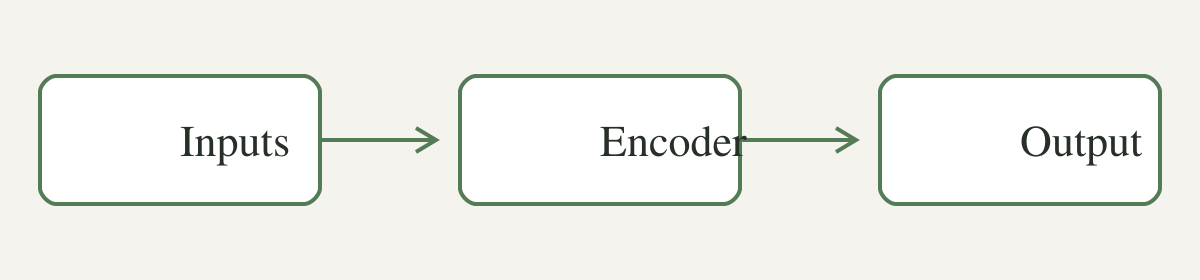
\includegraphics[width=0.8\linewidth]{figures/panel}
\caption{自制流程示意图，不代表真实模型结构或实测结果。}
\end{figure}
